%%%%%%%%%%%%%%%%%%%%%%%%%%%%%%%%%%%%%%%%%%%%%%%%%%%%%%%%%%%%%%%%%%%%%%%
% BAB 2
%%%%%%%%%%%%%%%%%%%%%%%%%%%%%%%%%%%%%%%%%%%%%%%%%%%%%%%%%%%%%%%%%%%%%%%

\mychapter{2}{BAB 2 LANDASAN KEPUSTAKAAN}



\section{Tinjauan Pustaka}

% comments
%% comments
Beberapa referensi digunakan dalam penelitian ini. 
\textcite{pramukantoroHeartbeatClassifierContinuous2022} telah mengusulkan beberapa algoritma untuk melakukan klasifikasi detak jantung dalam penelitiannya. 
Algoritma tersebut menggunakan RR-Interval dengan 9 deskriptor sebagai fiturnya.
Penelitian tersebut menggunakan metode \textit{machine learning Decision Tree, Gradient Boosting, k-Nearest Neighbors, Multi-layer Perceptron, Random Forest}, dan \textit{Support Vector Machine}, serta model \textit{deep learning} berupa \textit{Artificial Neural Network} (ANN). 
Penelitian tersebut mencapai nilai akurasi 99,31\% dengan menggunakan metode \textit{decision tree}, serta teknik \textit{random oversampling} untuk menambah jumlah sampel.
Selain itu, penelitian tersebut juga melakukan eksperimen implementasi inferensi secara \textit{realtime} untuk memprediksi kesehatan pasien dan mencapai hasil yang baik.

% Pada penelitian lain, \textcite{mondejar-guerraHeartbeatClassificationFusing2019} mengusulkan algoritma klasifikasi detak jantung dengan menggunakan fitur RR-Interval dengan 8 deskriptor. Dengan menggunakan fitur RR-Interval dan metode SVM, penelitian tersebut mendapatkan nilai akurasi 76,2\%. Penelitian tersebut juga menggunakan metode \textit{ensemble} SVM dengan fitur gabungan RR-Interval, wavelet, dan \textit{higher order statistics} (HOS) dan mendapat nilai akurasi 94,5\%.

Pada penelitian lain, \textcite{shchetininArrhythmiaDetectionUsing2022} telah melakukan penelitian untuk melakukan klasifikasi detak jantung dengan menggunakan metode \textit{deep learning} \textit{Long Short-Term Memory} (LSTM). 
Penelitian tersebut menggunakan dataset MIT-BIH Arrhythmia Database dan melakukan klasifikasi detak jantung menjadi 5 kelas, yaitu N, SVEB, VEB, F, dan Q.
Penelitian tersebut membuktikan bahwa metode LSTM digabungkan dengan teknik \textit{oversampling} SMOTE ENN dapat melakukan klasifikasi detak jantung dengan akurasi 97,22\%. 
% Pada penelitian lain, \textcite{shchetininArrhythmiaDetectionUsing2022} telah membuktikan bahwa metode LSTM dapat digunakan untuk melakukan klasifikasi detak jantung dan mendapatkan hasil yang baik.
% Penelitian tersebut melakukan klasifikasi detak jantung menjadi 5 kelas, yaitu N, SVEB, VEB, F, dan Q.

Pada penelitian sebelumnya, \textcite{sururiComparisonSeveralWavelet2023} telah melakukan perbandingan beberapa metode \textit{wavelet} sebagai metode ekstraksi fitur untuk inferensi klasifikasi detak jantung. 
Penelitian tersebut menggunakan metode \textit{wavelet Continuous Wavelet Transform} (CWT), \textit{Discrete Wavelet Transform} (DWT), dan \textit{Stationary Wavelet Transform} (SWT) untuk melakukan ekstraksi fitur dan digabungkan dengan metode \textit{deep learning Convolutional Neural Network} (CNN) untuk melakukan klasifikasi detak jantung menjadi 5 kelas.
Penelitian tersebut juga melakukan pengujian inferensi menggunakan dataset primer sepanjang 30 menit untuk mengevaluasi performa inferensi model klasifikasi detak jantung.
Penelitian tersebut mendapatkan hasil bahwa metode CWT memberikan nilai akurasi tertinggi, yaitu 99,08\%, namun memiliki waktu inferensi yang paling lama, yaitu 21,1326 detik dan penggunaan memori yang paling tinggi, yaitu 656,02 MB.
Sementara itu, metode DWT memberikan nilai akurasi terendah, yaitu 96,70\%, namun memiliki waktu inferensi tercepat, yaitu 12,9248 detik dan penggunaan memori terendah, yaitu 109,98 MB.


\section{Landasan Teori}

% \subsection{Detak Jantung}
% \label{subsec: landasan-detak-jantung}


% ectopic beats
\subsection{Detak \textit{Ectopic}}
\label{subsec: landasan-ectopic}

% Ectopic beats are extra beats that arise from an abnormal site that is different from the normal pacemaker of the heart (the sinus node). Ectopic beats can be thought of as extra electrical impulse that originate from an abnormal ‘switch’. Therefore, in a patient with ectopic beats, after every few beats from natural pacemaker (the sinus node ‘switch’), an extra beat will fire off from the abnormal site (ectopic ‘switch’). The extra beat typically occurs a short time after a normal beat and is therefore commonly referred to as a premature ectopic beat. In the majority of cases, the abnormal ‘switch’ fires off in a random fashion and therefore the heart does not beat in a synchronized fashion.
%
% Ectopic beats may arise from multiple locations in the heart. Extra beats that arise from the top chambers of the heart (atria) are called supraventricular ectopic beats (or premature supraventricular ectopic beats). Extra beats arising from the lower chambers (ventricles) are known as ventricular ectopic beats (or premature ventricular ectopic beats).

% Ectopic beats are abnormal beats that are due to unusual impulses. These abnormal excitations originate from atrio-ventricular junction or ventricles rather than the sino-atrial node. Ectopic beats can be seen in the ECG signal as abnormal waveforms.

% Ectopic heartbeats are changes in a heartbeat that is otherwise normal. These changes lead to extra or skipped heartbeats. 
% Ectopic beats may be caused or made worse by smoking, alcohol use, caffeine, stimulant medicines, and some street drugs.


Menurut kamus \textcite{merriam-websterDefinitionECTOPIC2024}, istilah \textit{ectopic} mengacu pada kejadian yang terjadi pada posisi yang tidak normal.
% Menurut kamus \textcite{merriam-websterDefinitionECTOPIC2024}, istilah \textit{ectopic} memiliki arti terjadi pada posisi yang tidak normal.
Detak \textit{ectopic} atau \textit{ectopic beats} adalah detak jantung abnormal yang terjadi di luar ritme detak jantung normal.
% Detak jantung normalnya dipacu secara alami oleh \textit{nodus sinoatrial} (SA).
Detak jantung normalnya dipacu oleh \textit{nodus sinoatrial} (SA), sebuah struktur di jantung yang berfungsi untuk memacu detak jantung secara alami.
Namun, detak \textit{ectopic} terjadi ketika impuls listrik yang memacu detak jantung bukan berasal dari SA, melainkan dari tempat lain di dalam jantung \parencite{mahidasaagarEctopicBeats}.
Detak \textit{ectopic} dapat berasal dari serambi jantung (atrium) maupun bilik jantung (ventrikel).
Detak \textit{ectopic} yang berasal dari atrium disebut dengan \textit{supraventricular ectopic beats}, sedangkan detak \textit{ectopic} yang berasal dari ventrikel disebut dengan \textit{ventricular ectopic beats}.
Detak \textit{ectopic} dapat dikenali melalui pola gelombang yang tidak normal pada sinyal \textit{electrocardiogram} (ECG).
% \subsubsection{\textit{Supraventricular Ectopic Beats} (SVEB)}
% \label{subsubsec: landasan-sveb}
%
% \subsubsection{\textit{Ventricular Ectopic Beats} (VEB)}
% \label{subsubsec: landasan-veb}

% mitbih

\subsection{\emph{Electrocardiogram} (ECG)}
\label{subsec: landasan-ecg}

\textit{Electrocardiogram} (ECG) merupakan uji kardiologi yang umum dilakukan untuk merekam aktivitas listrik jantung selama suatu periode dengan menggunakan elektroda \parencite{yoonDeepLearningbasedElectrocardiogram2019}.
Elektroda tersebut mendeteksi perubahan listrik kecil yang disebabkan oleh depolarisasi dan repolarisasi otot jantung pada tiap detaknya.
Hasil dari ECG tersebut berupa gelombang yang dapat digunakan untuk diagnosis medis.
ECG dapat digunakan untuk berbagai tujuan, seperti mengukur konsistensi, ukuran, dan lokasi denyut jantung serta untuk mengidentifikasi kerusakan jantung.


Gambar \ref{fig: ecg-morphology} menunjukkan morfologi gelombang ECG. ECG terdiri dari beberapa komponen: gelombang P, kompleks QRS, dan gelombang T, serta durasi antara komponen tersebut \parencite{anbalaganAnalysisVariousTechniques2023}.  Gelombang P menunjukkan depolarisasi atrium, kompleks QRS menunjukkan depolarisasi ventrikel, dan gelombang T menunjukkan repolarisasi ventrikel.

\begin{figure}[H]
  \centering
  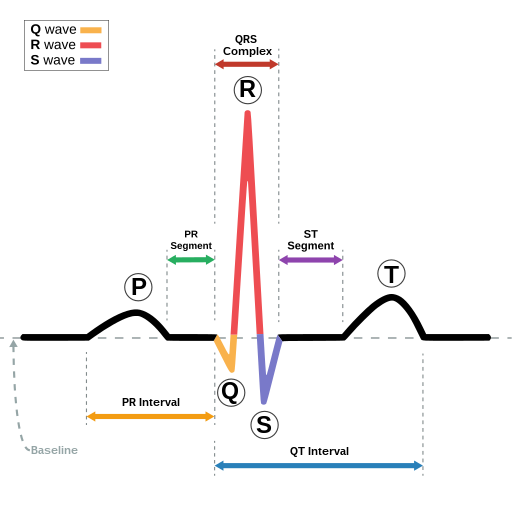
\includegraphics[width=.5\linewidth]{img/ecg-morphology.png}
  \caption{Morfologi gelombang ECG}
  Sumber: \textcite{wiki:xxx}
  \label{fig: ecg-morphology}
\end{figure}

\subsection{\textit{MIT-BIH Arrhythmia Database}}
\label{subsec: landasan-mitbih}

% \textit{MIT-BIH Arrhythmia Database} adalah dataset publik yang berisi rekaman ECG dari 47 pasien yang berdurasi 30 menit \parencite{moodyImpactMITBIHArrhythmia2001}.
\textit{MIT-BIH Arrhythmia Database} merupakan salah satu dataset publik yang dikembangkan oleh \textit{Massachusetts Institute of Technology} (MIT) dan \textit{Beth Israel Hospital} (BIH) \parencite{moodyImpactMITBIHArrhythmia2001}.
Dataset ini berisi 48 rekaman ECG dari 47 pasien yang masing-masing berdurasi 30 menit dan terdiri dari dua kanal.
Dari 48 rekaman tersebut, data 102, 104, 107, dan 217 berisi data detak jantung yang sedang dipacu.
Dataset ini direkam dengan frekuensi 360 Hz dan resolusi 11-bit.
Setiap detak jantung pada dataset, telah diberi label dan anotasi oleh para ahli.
% Pemberian label pada detak jantung dilakukan dengan menggunakan simbol-simbol tertentu.
% Simbol-simbol tersebut dideskripsikan pada tabel \ref{tab:beat_symbols}.
Pemberian label dilakukan menggunakan simbol-simbol tertentu yang dijelaskan dalam Tabel \ref{tab:beat_symbols}.

% tabel simbol yang digunakan pada dataset

% Symbol	Meaning
% · or N	Normal beat
% L	Left bundle branch block beat
% R	Right bundle branch block beat
% A	Atrial premature beat
% a	Aberrated atrial premature beat
% J	Nodal (junctional) premature beat
% S	Supraventricular premature beat
% V	Premature ventricular contraction
% F	Fusion of ventricular and normal beat
% [	Start of ventricular flutter/fibrillation
% !	Ventricular flutter wave
% ]	End of ventricular flutter/fibrillation
% e	Atrial escape beat
% j	Nodal (junctional) escape beat
% E	Ventricular escape beat
% /	Paced beat
% f	Fusion of paced and normal beat
% x	Non-conducted P-wave (blocked APB)
% Q	Unclassifiable beat
% |	Isolated QRS-like artifact

\begin{table}[H]
    \centering
    \caption{Deskripsi simbol pada \textit{MIT-BIH Arrhythmia Database}}
    \begin{tabular}{|c|l|}
    \hline
    \textbf{Simbol} & {\centering \textbf{Deskripsi}} \\
    \hline
    % $\cdot$ or N & Normal beat \\
    $\cdot$ atau N & Denyut normal \\
    % L & Left bundle branch block beat \\
    L & Denyut \textit{left bundle branch block} (LBBB) \\
    % R & Right bundle branch block beat \\
    R & Denyut \textit{right bundle branch block} (RBBB) \\
    % A & Atrial premature beat \\
    A & \textit{Atrial premature beat} (APB) \\
    % a & Aberrated atrial premature beat \\
    a & \textit{Aberrated atrial premature beat} \\
    % J & Nodal (junctional) premature beat \\
    J & \textit{Nodal (junctional) premature beat} \\
    % S & Supraventricular premature beat \\
    S & \textit{Supraventricular premature beat} \\
    % V & Premature ventricular contraction \\
    V & \textit{Premature ventricular contraction} (PVC) \\
    % F & Fusion of ventricular and normal beat \\
    F & Gabungan denyut ventrikel dan normal \\
    % {[} & Start of ventricular flutter/fibrillation \\
    {[} & Awal dari \textit{ventricular flutter/fibrillation} \\
    % ! & Ventricular flutter wave \\
    ! & \textit{Ventricular flutter wave} \\
    % {]} & End of ventricular flutter/fibrillation \\
    {]} & Akhir dari \textit{ventricular flutter/fibrillation} \\
    % e & Atrial escape beat \\
    e & \textit{Atrial escape beat} \\
    % j & Nodal (junctional) escape beat \\
    j & \textit{Nodal (junctional) escape beat} \\
    % E & Ventricular escape beat \\
    E & \textit{Ventricular escape beat} \\
    % / & Paced beat \\
    / & Denyut yang dipacu \\
    % f & Fusion of paced and normal beat \\
    f & Gabungan denyut dipacu dan normal \\
    % x & Non-conducted P-wave (blocked APB) \\
    x & Gelombang P yang tidak terkonduksi \\
    % Q & Unclassifiable beat \\
    Q & Denyut yang tidak dapat diklasifikasikan \\
    % | & Isolated QRS-like artifact \\
    \hline
    \end{tabular} \\
    \vspace{0.5em}
    Sumber: \textcite{moodyImpactMITBIHArrhythmia2001}
    \label{tab:beat_symbols}
\end{table}

\subsection{\textit{Long Short-Term Memory} (LSTM)}
\label{subsec: landasan-lstm}

\textit{Long Short-Term Memory} atau dapat disingkat LSTM merupakan pengembangan dari metode \textit{deep learning Recurrent Neural Network} (RNN). LSTM dirancang untuk mengatasi salah satu masalah yang umum terjadi pada RNN tradisional, yaitu hilangnya informasi masa lalu \parencite{hochreiterLongShorttermMemory1997}. Metode LSTM dapat diterapkan pada klasifikasi, pengolahan, dan prediksi berdasarkan data sekuensial, seperti teks dan suara,  termasuk juga data yang terkait dengan bidang kesehatan.

\begin{figure}[H]
  \centering
  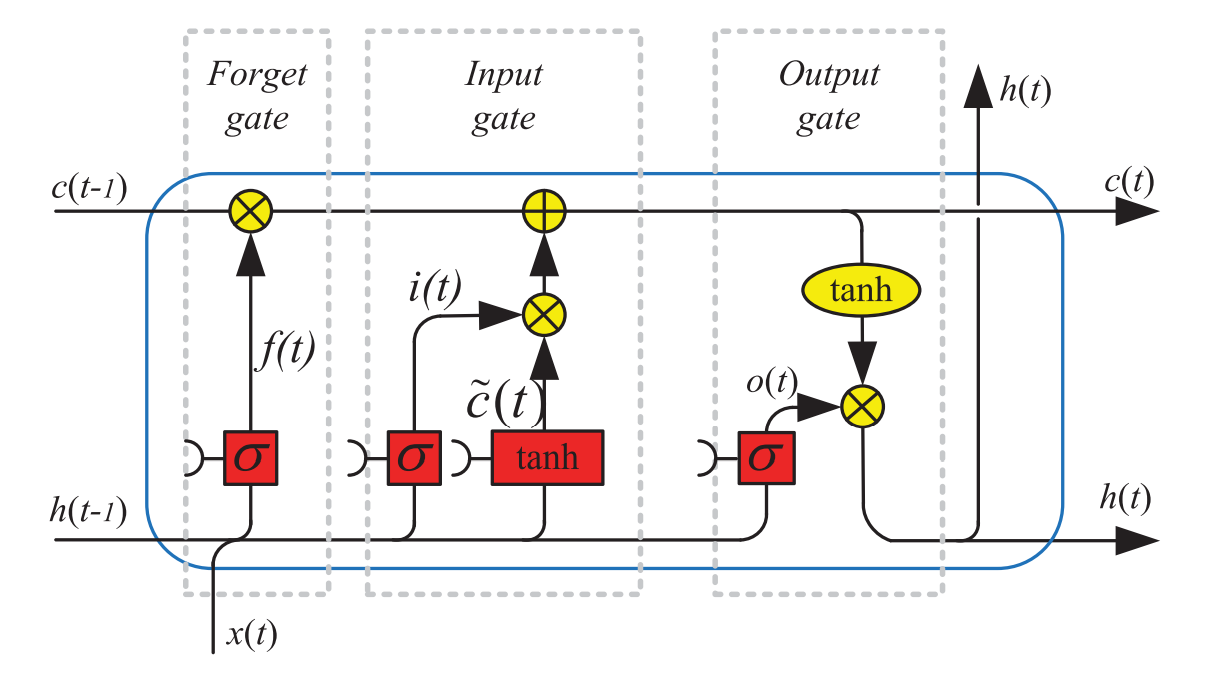
\includegraphics[width=.7\linewidth]{img/ecg-arch.png}
  \caption{Arsitektur sel LSTM}
  Sumber: \textcite{yuReviewRecurrentNeural2019}
  \label{fig:arsitektur-lstm}
\end{figure}

Gambar \ref{fig:arsitektur-lstm} menunjukkan arsitektur sel LSTM. Sebuah sel LSTM umumnya terdiri dari tiga buah \textit{gate}, yaitu \textit{input gate, output gate}, dan \textit{forget gate}. Ketiga gate tersebut berfungsi untuk mengatur informasi yang masuk maupun keluar dari sel LSTM.
\textit{Input gate} menentukan informasi baru yang akan disimpan pada \textit{cell state} (Ct), \textit{output gate} menentukan informasi apa yang akan jadi output, dan \textit{forget gate} menentukan informasi apa yang akan dibuang dari \textit{cell state} \parencite{yuReviewRecurrentNeural2019}.

Berdasarkan gambar \ref{fig:arsitektur-lstm}, secara matematis LSTM dapat didefinisikan dengan persamaan \ref{def-lstm}.
\begin{equation}
\begin{split}
    f_t &= \sigma (W_{fh}h_{t-1} + W_{fx}x_t + b_f), \\
    i_t &= \sigma (W_{ih}h_{t-1} + W_{ix}x_t + b_i),\\
    \tilde{c}_t &= \tanh (W_{\tilde{c}h}h_{t-1} + W_{\tilde{c}x}x_t + b_{\tilde{c}}), \\
    c_t &= f_t \cdot c_{t-1}+ i_t \cdot \tilde{c}_t,\\
    o_t &= \sigma (W_{oh}h_{t-1} + W_{ox}x_t + b_o), \\
    h_t &= o_t \cdot \tanh(c_t).
\end{split}
    \label{def-lstm}
\end{equation}
\noindent
Di mana \(f_t\), \(i_t\), \(o_t\) dan \(c_t\) masing-masing menunjukkan nilai \emph{forget gate}, \emph{input gate}, \emph{output gate}, dan \emph{cell state}.

% \subsection{Raspberry Pi 3}
% \label{subsec: landasan-raspi}
%
% %raspi secara umum
% Raspberry Pi merupakan sebuah komputer mini seukuran kartu kredit yang dikembangkan oleh Raspberry Pi Foundation \parencite{8756967}. 
% Raspberry Pi memiliki beberapa kelebihan, seperti ukurannya yang kecil, konsumsi daya yang rendah, harga yang terjangkau, serta kemampuan komputasi baik.
% %need citation
% Raspberry Pi dapat diaplikasikan pada berbagai bidang, seperti industri, agrikultur, bioteknologi, dan kesehatan \parencite{9760691}.
%
% %raspi 4 
% %*sekara sudah bukan yang terbaru, sudah ada raspi 5
% % Raspberry Pi 4 model B merupakan salah satu varian dari Raspberry Pi generasi keempat. Raspberry Pi 4 model B memiliki spesifikasi prosesor \textit{quad-core} ARM Cortex-A72 1.5GHz, dengan pilihan RAM 2GB, 4GB, atau 8GB LPDDR4-3200 SDRAM. Raspberry Pi 4 model B juga dilengkapi dengan konektivitas WiFi 2.4GHz dan 5GHz, Bluetooth 5.0, serta \textit{ethernet} dengan kecepatan maksimum 1Gbps. Raspberry Pi 4 model B juga memiliki \textit{port micro} HDMI, USB 3.0, USB 2.0, dan port GPIO.
%
% % raspi 3
% % Pengujian dilakukan pada perangkat Raspberry Pi 3B. Perangkat ini memiliki prosesor ARMv8 quad-core 1,2GHz dan RAM 1GB LPDDR2. Konektivitas perangkat ini didukung dengan 2.4Ghz WiFi serta \textit{ethernet} dengan kecepatan maksimum 100Mbps.
% Raspberry Pi 3 merupakan salah satu varian dari Raspberry Pi generasi ketiga. Raspberry Pi 3 memiliki spesifikasi prosesor ARMv8 \textit{quad-core} 1,2GHz dan RAM 1GB LPDDR2. Raspberry Pi 3 juga telah dilengkapi dengan konektivitas WiFi 2.4GHz dan \textit{ethernet} dengan kecepatan maksimum 100Mbps. Raspberry Pi 3 juga memiliki \textit{port} HDMI, USB 2.0, dan \textit{port} GPIO.

% klasifikasi detak jantung
% tentang detak jantung menurut AAMI

% heart related disease class
% N, sveb, veb, f, dan q
% \section{Klasifikasi Detak Jantung}

% \section{Inferensi}

% metrik evaluasi
% akurasi, presisi, recall, f1-score

% TODO
% landasan teori lain
% penerapan lstm di edge device

